\input ../SlidePreamble
\input ../preamble

\begin{document}

{\Huge

  \centerline{\bf TTIC 31230, Fundamentals of Deep Learning}
  \bigskip
  \centerline{David McAllester, Winter 2020}

  \vfill
  \centerline{\bf What About alpha-beta?}
  \vfill
  \vfill

\slide{Grand Unification}

AlphaZero unifies chess and go algorithms.

\vfill
This unification of intuition (go) and calculation (chess) is surprising.

\vfill
This unification grew out of go algorithms.

\vfill
But are the algorithmic insights of chess algorithms really irrelevant?

\slide{Chess Background}

The first min-max computer chess program was described by Claude Shannon in 1950.

\vfill
Alpha-beta pruning was invented by various people independently, including John McCarthy in the late 1950s.

\vfill
Alpha-beta has been the cornerstone of all chess algorithms until AlphaZero.


\slide{Alpha-Beta Pruning}

\begin{verbatim}
def MaxValue(s,alpha,beta):
   value = alpha
   for s2 in s.children():
     value = max(value, MinValue(s2,value,beta))
     if value >= beta: break()
   return value

def MinValue(s,alpha,beta):
   value = beta
   for s2 in s.children():
     value = min(value, MaxValue(s2,alpha,value))
     if value <= alpha: break()
   return value
\end{verbatim}

\slideplain{Strategies}


An optimal alpha-beta tree is the union of a root-player strategy and an opponent strategy.

\vfill
A strategy for the root player is a selection of a single action for each root-player move and a response for each possible action
of the opponent.

\vfill
A strategy for the opponent is a selection of a single action for each opponent move and a response for each possible action
of the root player.

\slide{Proposal}

Simulations should be divided into root-player strategy simulations and opponent strategy simulations.

\vfill
A root-player strategy simulation is optimistic for the root player and pessimistic for the opponent.

\vfill
An opponent strategy simulation is optimistic for the opponent player and pessimistic for the root-player.

\slide{Proposal}

$$U(s,a) =  \left\{\begin{array}{ll}\lambda_u \; \pi_\Phi(s,a) &\mbox{if $N(s,a) = 0$}
\\ \hat{\mu}(s,a) + \lambda_u\; \pi_\Phi(s,a)/N(s,a) & \mbox{otherwise} \end{array}\right. \;\;\;\;(1)$$

\vfill
$\lambda_u$ should be divided into $\lambda_u^+$ and $\lambda_u^-$ with $\lambda_u^+ > \lambda_u^-$.

\vfill
Simulations should be divided into two types --- optimistic and pessimistic.

\vfill
In optimistic simulations we use $\lambda_u^+$ for root-player moves and $\lambda_u^-$ for opponent moves.

\vfill
In pessimistic simulations we use $\lambda_u^-$ for root-player moves and $\lambda_u^+$ for opponent moves.

\slide{AlphaStar}

Grandmaster level in StarCraft II using multi-agent reinforcement learning, Nature Oct. 2019, Vinyals et al.

\vfill
StarCraft:

\begin{itemize}
\item Players control hundreds of units.

\vfill
\item Individual actions are selected from $10^{26}$ possibilities (an action is a kind of procedure call with arguments).

\vfill
\item Cyclic non-transitive strategies (rock-paper-scisors).

\vfill
\item Imperfect information --- the state is not fully observable.
\end{itemize}

\slide{The Paper is Vague}

It basically says the following ideas are used:

A policy gradient algorithm, auto-regressive policies, self-attention over the observation history, LSTMs, pointer-networks, scatter connections,
replay buffers, asynchronous advantage actor-critic algorithms, TD($\lambda$) (gradients on value function Bellman error), clipped importance sampling
(V-trace), a new undefined method they call UPGO that ``moves policies toward trajectories with better than average reward'', a value function
that can see the opponents observation (training only), a ``$z$ statistic'' stating a high level strategy, 
supervised learning from human play, 
a ``league'' of players (next slide).

\slide{The League}

The league has three classes of agents: main (M), main exploiters (E), and league exploiters (L).  M and L play against everybody.
E plays only against M.

\slide{A Rube Goldberg Contraption?}

\centerline{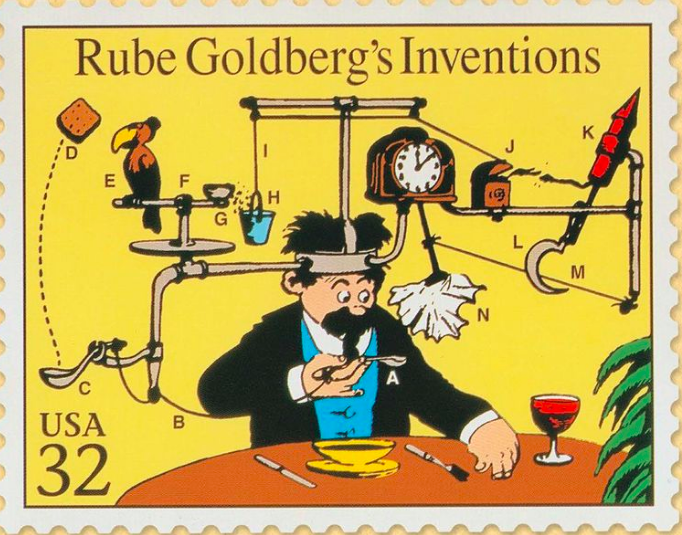
\includegraphics[height = 5in]{\images/Goldberg}}

\slide{Video}

https://www.youtube.com/watch?v=UuhECwm31dM

\slide{END}



}
\end{document}

\ignore{
\slideplain{Conspiracy Numbers}

Conspiracy Numbers for Min-Max search, McAllester, 1988

\vfill
Each node $s$ has a min-max value $V(s)$ determined by the leaf values.

\vfill
For any positive integer $N$ and potential value $V$ we define $L(N,V)$ to be the set of leaf nodes $s_1$ such that
there exist $N-1$ other leaf nodes $s_2$, $\ldots$, $s_N$ such that by changing the values of $s_1$, $\ldots$, $s_N$ the root node
can be changed to $V$.


\vfill
{\bf Algorithm:}


\vfill
Repeatedly select some $N$ and $V$ such that $L(N,V)$ is non empty and expand some leaf in $L(N,V)$.
}

\ignore{
\slide{Simulation}

To find an upper-confidence leaf for the root and value $U$:

\vfill
At a max node pick the child minimizing $N(s,U)$.

\vfill
At a min node select any child $s$ with $V(s) < U$.

\vfill
\slide{Refinement}

Let the static evaluator associate leaf nodes with values $U(s,N)$ and $L(s,N)$
}

